\documentclass[11pt]{article}
\usepackage{listings}
\lstset{language=Matlab,
breaklines=true,
keywordstyle=\color{blue},
identifierstyle=\color{black},
stringstyle=\color{mylilas},
commentstyle=\color{mygreen},
showstringspaces=false,
numbers=left,
numberstyle={\small \color{black}},
numbersep=9pt,
emph=[1]{for,end,break},
emphstyle=[1]\color{red}
}

\usepackage{color}
\definecolor{mygreen}{RGB}{28,172,0}
\definecolor{mylilas}{RGB}{170,55,241}

\usepackage{fancyhdr}
\pagestyle{fancy}
\newcommand\course{CSC 349A}
\newcommand\hwnumber{3}
\newcommand\duedate{October 8, 2019}

\lhead{Oliver Tonnesen\\V00885732}
\chead{\textbf{\Large Assignment \hwnumber}}
\rhead{\course\\\duedate}

\usepackage{graphicx}

\usepackage{amsmath}
\DeclareMathOperator{\fl}{fl}


\begin{document}
\renewcommand{\thesubsection}{\thesection.\alph{subsection}}
\section{} % Section 1
\subsection{} % Section 1.a
\begin{align*}
	\fl(f(x))&=\fl\Biggl(\frac{\fl\bigl(1+\fl(\cos{3.155})\bigr)}{\fl\bigl(\fl\bigl(3.155-\fl(\pi)\bigr)^2\bigr)}\Biggr)\\
	&=\fl\Biggl(\frac{\fl\bigl(1+(-0.9999)\bigr)}{\fl\bigl(0.01300\bigr)^2}\Biggr)\\
	&=\fl\Biggl(\frac{0.0001000}{0.0001690}\Biggr)\\
	&=0.5917
\end{align*}
Note that $\vert\varepsilon_t\vert=\vert1-\frac{0.5917}{0.49999251}\vert\approx0.1834>0.1$,
as desired.


\subsection{} % Section 1.b
\begin{align*}
	\cos x&\approx\cos\pi-\sin\pi(x-\pi)-\frac{\cos\pi}{2}(x-\pi)^2+\frac{\sin\pi}{6}(x-\pi)^3+\frac{\cos\pi}{24}(x-\pi)^4\\
	&=-1+\frac{(x-\pi)^2}{2}-\frac{(x-\pi)^4}{24}
\end{align*}


\subsection{} % Section 1.c
\begin{align*}
	f(x)&\approx\frac{1+(-1+\frac{(x-\pi)^2}{2}-\frac{(x-\pi)^4}{24})}{(x-\pi)^2}\\
	&=\frac{1}{2}-\frac{(x-\pi)^2}{24}
\end{align*}


\subsection{} % Section 1.d
Let $\varepsilon$ such that $\vert\frac{\varepsilon}{3.155}\vert$ is small. We
know that $\frac{1}{2}-\frac{(x-\pi)^2}{24}$ is a very good approximation for
$f(x)$, so consider $\frac{1}{2}-\frac{(x+\varepsilon-\pi)^2}{24}$:
\begin{align*}
	\frac{1}{2}-\frac{(x+\varepsilon-\pi)^2}{24}&\approx
	\frac{1}{2}-\frac{(0.01341+\varepsilon)^2}{24}.
\end{align*}
We assume ``small'' here means $\vert\frac{\varepsilon}{3.155}\vert<0.01$, so
$0.49999983\le\frac{1}{2}-\frac{(0.01341+\varepsilon)^2}{24}\le0.499999996$.
In other words, the function evaluated at any small perturbation
$x+\varepsilon$ of $x$ gives a value very close to the exact value of the
function when evaluated at $x$, so the problem of computing $f(3.155)$ is
well-conditioned.


\subsection{} % Section 1.e
Again, we use our approximation to $f(x)$, $\frac{1}{2}-\frac{(x-\pi)^2}{24}$.
Let $\varepsilon$ such that $\vert\frac{\varepsilon}{3.155}\vert<0.01$. Then
\begin{align*}
	\fl\Biggl(\frac{1}{2}-\frac{\fl(\fl(\fl(3.155-\pi)+\varepsilon)^2)}{24}\Biggr)
	&=\fl\Biggl(\frac{1}{2}-\frac{\fl((0.013+\varepsilon)^2)}{24}\Biggr)
\end{align*}
and $0.4999\le\fl\Bigl(\frac{1}{2}-\frac{\fl((0.013+\varepsilon)^2)}{24}\Bigr)\le0.5$.
So clearly no small perturbation $x+\varepsilon$ of $x$ will give a value close
to the calculated value of 0.5917 in a).


\section{} % Section 2
\subsection{} % Section 2.a
\lstinputlisting{mfiles/Bisect.m}


\subsection{} % Section 2.b
We have that
\begin{align*}
	B=2+y\\
\end{align*}
	and
\begin{align*}
	A_c=2y+\frac{y^2}{2},
\end{align*}
so since it must always be the case that
\begin{align*}
	0=1-\frac{Q^2}{gA_c^3}B,
\end{align*}
we can simply find the roots of the function
\begin{align*}
	f(y)&=1-\frac{Q^2}{gA_c^3}B\\
	&=1-\frac{Q^2}{g(2y+\frac{y^2}{2})^3}(2+y)\\
	&=1-\frac{18^2}{9.81(2y+\frac{y^2}{2})^3}(2+y)
\end{align*}



\subsection{} % Section 2.c
Below is the additional M-file:
\lstinputlisting{mfiles/q2c.m}
The MATLAB statements used to call Bisect, along with its output:
\lstinputlisting[numbers=none]{mfiles/Q2c}
Finally, below is the figure produced by the above call to Bisect:
\centering
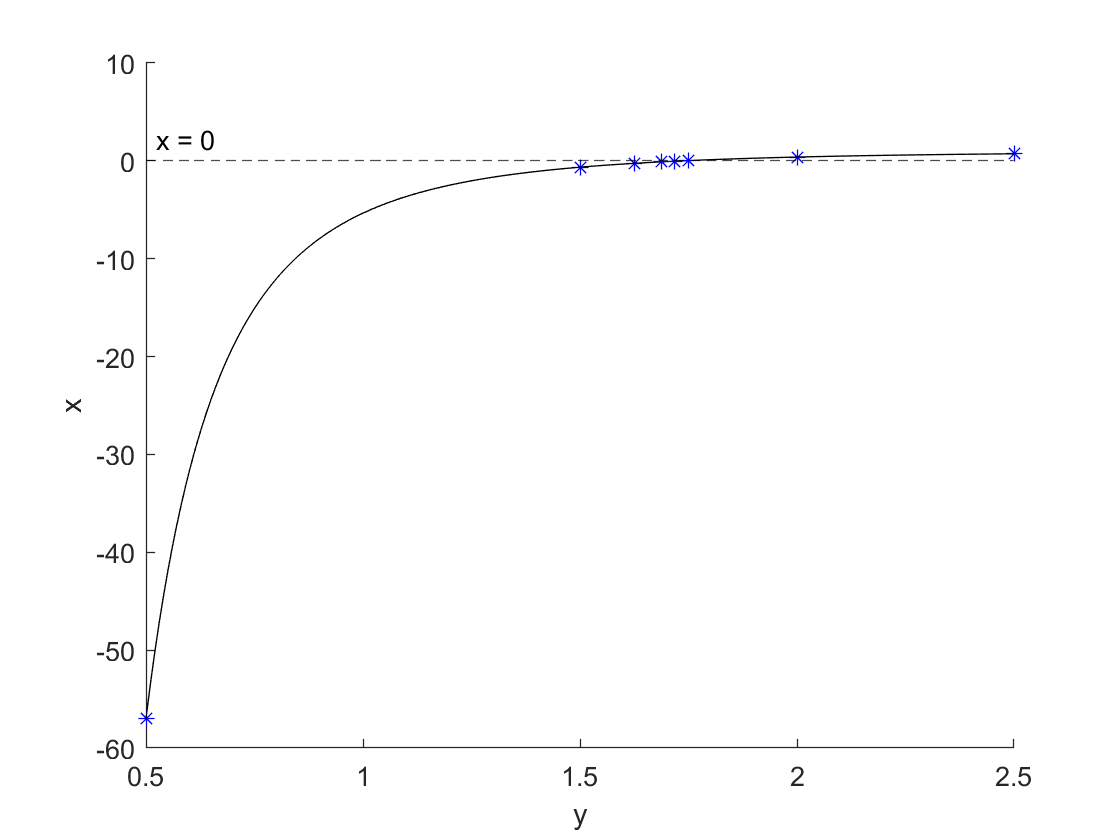
\includegraphics[scale=0.45]{q2c.png}


\end{document}
